\sf\Large

%\centerline{\underline{\Huge\bf ДВИЖЕНИЕ ЖИДКОСТИ}}

\underline{\bf Сплошная среда \sl(continuum)}: непрерывное $\infty$ тело, в котором воз\-мо\-ж\-но перемещение различных частей относительно друг друга.
\begin{itemize}
\item Упругое тв. тело: относительные сдвиги, колебания
\item Несжимаемая жидкость: течения
\item Сжимаемая жидкость или газ: течения, колебания
\end{itemize}
Гидродинамика -- часть механики, изучающая движение жидкостей.\\
{\color{blue}Идеальная жидкость} -- несжимаемая и без вязкости (нет внутреннего трения)\\
  \begin{picture}(190,25)(0,0)
   %\put(0,0){\framebox(190,25)[b]{}}
   \put(135,0){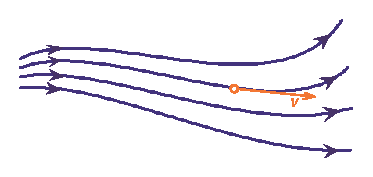
\includegraphics{GP006/GP006F01.eps}}
   \put(0,22){\makebox(0,0)[tl]{\parbox{130mm}{
   {\color{blue}Поле вектора скорости}: пространство, где можно провести {\color{blue}линии тока} -- касательные к ним в каждой точке совпадают с направлением скорости частиц
   }}}
  \end{picture}\\[10mm]
  \begin{picture}(190,25)(0,0)
   %\put(0,0){\framebox(190,25)[b]{}}
   \put( 10,0){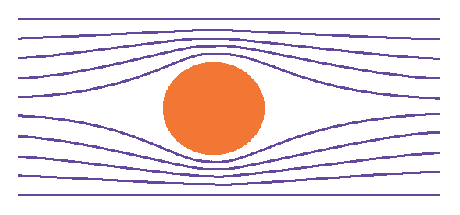
\includegraphics{GP006/GP006F2a.eps}}
   \put(100,0){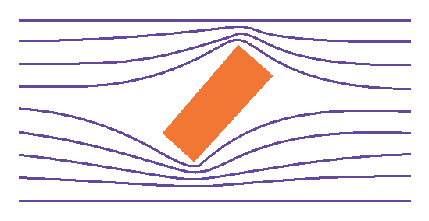
\includegraphics{GP006/GP006F2b.eps}}
  \end{picture}\\[5mm]
  \begin{picture}(190,52)(0,0)
   %\put(0,0){\framebox(190,50)[b]{}}
   \put( 125,0){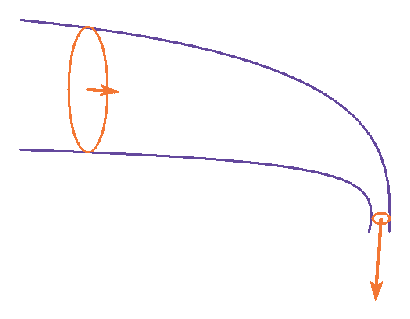
\includegraphics{GP006/GP006F03.eps}}
   {\color{red}
   \put(129,40){\makebox(0,0)[l]{$\Delta S_1$}}
   \put(143,35){\makebox(0,0)[l]{$\vec{v}_1$}}
   \put(183,15){\makebox(0,0)[r]{$\Delta S_2$}}
   \put(184,5){\makebox(0,0)[r]{$\vec{v}_2$}}
   }
   \put(0,52){\makebox(0,0)[tl]{\parbox{120mm}{
  Часть жидкости, ограниченная линиями тока -- {\color{blue} трубка тока}. Линии тока образуют как бы невидимые границы: частицы жидкости их не пересекают (иначе скорость была бы направлена по-другому).  }}}
   \put(0,0){\makebox(0,0)[bl]{\parbox{165mm}{
   Если в трубке тока провести 2 нормальных сечения $\Delta S_1$ и $\Delta S_2$, то за единицу времени через $\Delta S_1$ протечет объем =$\Delta S_1\cdot v_1$. Если
  }}}
  \end{picture}\\
  жидкость несжимаема, то через $\Delta S_2$ протечет столько же: $\Delta S_2\cdot v_2=\Delta S_1\cdot v_1$, и вообще для данной трубки
  \begin{displaymath}
\Delta S\cdot v=\texttt{const}\hspace{10mm}\texttt{\color{blue} -- теорема о неразрывности струи}
  \end{displaymath}

  Если $\exists$ реальная труба, то ее внутренний объем -- трубка тока. Тогда: где труба \'{у}же, там течение быстрее.
Если трубка сужается, то скорость возрастает $\Rightarrow$ есть ускорение $\Rightarrow$ есть сила! Откуда? От разности давлений. Давление в широких местах > чем в узких.

%\newpage
  \noindent
  \begin{picture}(190,60)(0,0)
   %\put(0,0){\framebox(190,60)[b]{}}
   \put( 100,0){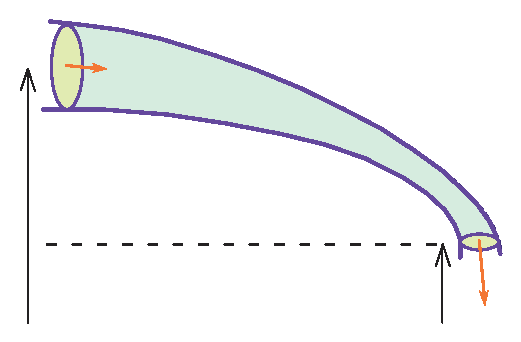
\includegraphics{GP006/GP006F04.eps}}
   {\color{red}
   \put(110,52){\makebox(0,0)[b]{$S_1$}}
   \put(188,17){\makebox(0,0)[r]{$S_2$}}
   \put(115,40){\makebox(0,0)[l]{$\vec{v}_1$}}
   \put(186,5){\makebox(0,0)[r]{$\vec{v}_2$}}
   \color{blue}
   \put(117,47){\makebox(0,0)[r]{$p_1$}}
   \put(176,18){\makebox(0,0)[c]{$p_2$}}
   }
   \put(100,5){\makebox(0,0)[r]{$h_1$}}
   \put(170,5){\makebox(0,0)[r]{$h_2$}}
   \put(103,20){\makebox(0,0)[lb]{$h = h_1-h_2$}}
   \put(0,60){\makebox(0,0)[tl]{\parbox{90mm}{
   $S_{1,2}$ -- сечение\\
   $\vec{v}_{1,2}$ -- скорость\\
   $p_{1,2}$ -- давление\\
   $h_{1,2}$ -- высота\\
   $m$ -- порция жидкости (масса)\\
   $E_{1,2}$ -- полная энергия порции\\
   $A$ -- работа по перемещению $m$\\ от сечения 1 до сечения 2
  }}}
  \end{picture}\\
\begin{displaymath}
A=E_2-E_1,\;\;\;\;\;\;\;\;E_{1,2}=E_\texttt{кин}+E_\texttt{пот}
\end{displaymath}
\begin{displaymath}
E_1=\frac{m\cdot v_1^2}2+mgh_1\;\;\;\;\;\;\;E_2=\frac{m\cdot v_2^2}2+mgh_2
\end{displaymath}
Пусть весь столб жидкости сдвигается за время $t$ так, что через оба сечения проходит порция $m$. В точке (1) это смещение $L_1=v_1t$, а в точке (2) -- $L_2=v_2t$. Сила, толкающая жидкость в точке (1) -- это $f_1=p_1S_1$, а сила, сопротивляющаяся движению в точке (2) -- это $f_2=-p_2S_2$ (знак "минус" именно потому, что давление $p_2$ направлено навстречу движению). Работа внешних сил
\begin{displaymath}
A=f_1L_1+f_2L_2=p_1S_1v_1t-p_2S_2v_2t.
\end{displaymath}
Приравняв $A$ и $E_2-E_1$, получим:
\begin{displaymath}
\frac{m\cdot v_2^2}2+mgh_2-\frac{m\cdot v_1^2}2-mgh_1=p_1S_1v_1t-p_2S_2v_2t.
\end{displaymath}или
\begin{equation}\label{eqn.2}
 \frac{m\cdot v_1^2}2+mgh_1+p_1S_1v_1t=\frac{m\cdot v_2^2}2+mgh_2+p_2S_2v_2t.
\end{equation}
По закону неразрывности струи: $S_1v_1t=S_2v_2t$, и это -- объем $V$, занимаемый порцией $m$. Поделим ур-ние (\ref{eqn.2}) на $V$ и учтем, что $\frac mV$ -- это плотность $\rho$:
{\color{blue}
\begin{displaymath}
\frac{\rho\cdot v_1^2}2+\rho gh_1+p_1=\frac{\rho\cdot v_2^2}2+\rho gh_2+p_2.
\end{displaymath}
}
\begin{flushright}{\sl Даниил БЕРНУЛЛИ (1700-1782), СПб}\end{flushright}

%\newpage
  \noindent
  \begin{picture}(190,40)(0,0)
   %\put(0,0){\framebox(190,40)[b]{}}
   \put(20,0){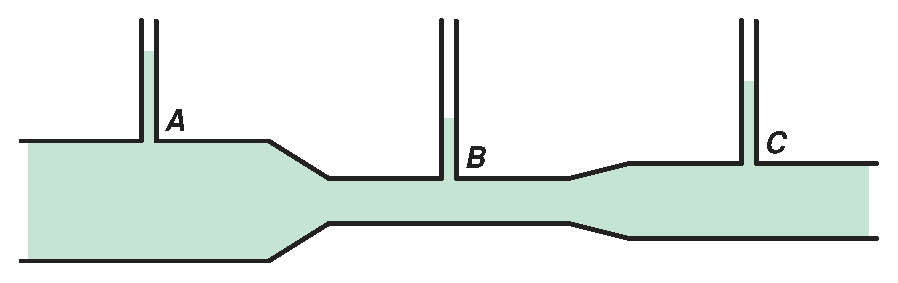
\includegraphics{GP006/GP006F05.eps}}
  \end{picture}
\begin{displaymath}
\frac{\rho\cdot v_A^2}2+p_A
\hspace{7mm}=
\hspace{7mm}\frac{\rho\cdot v_B^2}2+p_B
\hspace{7mm}=
\hspace{7mm}\frac{\rho\cdot v_C^2}2+p_C
\end{displaymath}\\
\rule{189mm}{0.3mm}\\
  \begin{picture}(190,50)(0,0)
   %\put(0,0){\framebox(190,50)[b]{}}
   \put(80,0){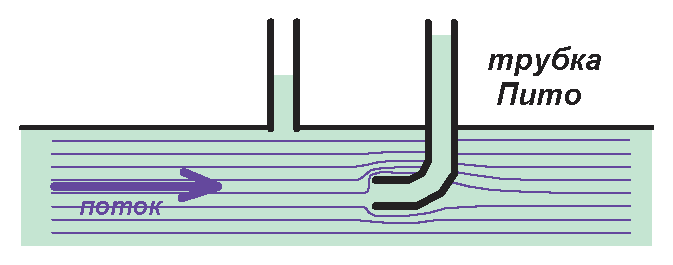
\includegraphics{GP006/GP006F06.eps}}
   {\color{blue}
   \put(121,30){\makebox(0,0)[r]{$p_1$}}
   \put(148,30){\makebox(0,0)[r]{$p_2$}}
   }
   \put(5,45){\makebox(0,0)[tl]{\parbox{97mm}{
Скорость жидкости непосредственно перед отверстием трубки Пито $v_2=0$.
\begin{displaymath}
p_2=\frac{\rho\cdot v_1^2}2+p_1
\end{displaymath}
$p_2$ -- {\color{red} динамическое давление}
   }}}
  \end{picture}\\[2mm]
$p_1,p_2\;\;\;\Rightarrow$ измерение скорости жидкости (флот) или газа (авиация) по разности давлений.\\
\rule{189mm}{0.3mm}\\

Струйный насос:\\
  \begin{picture}(190,60)(0,0)
   %\put(0,0){\framebox(190,60)[b]{}}
   \put(0,0){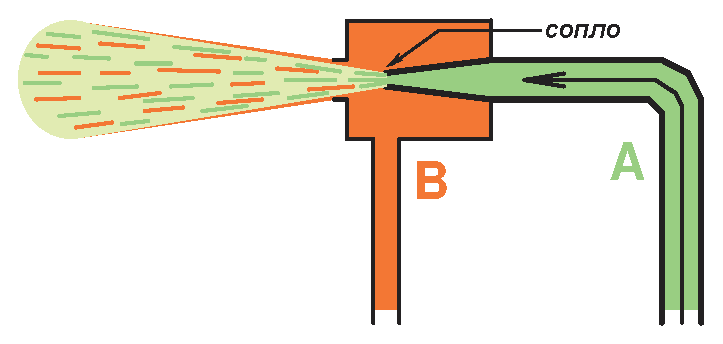
\includegraphics{GP006/GP006F07.eps}}
   \put(190,60){\makebox(0,0)[tr]{\parbox{70mm}{
При достаточно большой скорости жидкости {\bf \color{green}A} на выходе из сопла давление там может стать < ат\-мо\-сфер\-но\-го, и жидкость {\bf \color{red}B} будет засасываться в струю. (жидкость $\Leftrightarrow$ газ)
   }}}
  \end{picture}\\
  \begin{picture}(190,60)(0,0)
   %\put(0,0){\framebox(190,60)[b]{}}
   \put(0,0){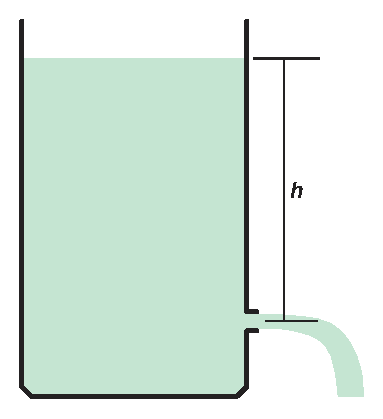
\includegraphics{GP006/GP006F08.eps}}
   \put(190,60){\makebox(0,0)[tr]{\parbox{130mm}{
Весь сосуд -- как одна трубка тока. Давление и у поверхности, и у отверстия = атмосферному.
Уравнение Бернулли:
\begin{displaymath}
\frac{v_1^2}2+g(h_1-h_2)=\frac{v_2^2}2
\end{displaymath}
Поскольку скорость у поверхности $\simeq0$, то получим:
\begin{displaymath}
v_2=\sqrt{2g(h_1-h_2)}=\sqrt{2gh}
\end{displaymath}
   }}}
  \end{picture}\\

Закон сохранения количества движения: струя приобрела скорость вправо; если бы система была замкнутой, то сосуд двинулся бы влево.\\ \\
  \begin{picture}(190,60)(0,0)
   %\put(0,0){\framebox(190,60)[b]{}}
   \put(0,0){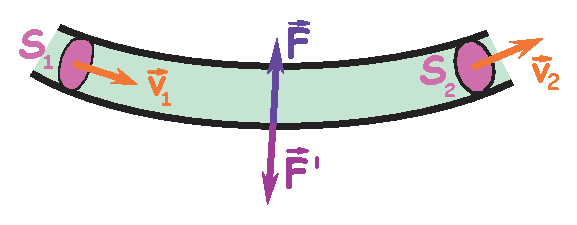
\includegraphics{GP006/GP006F09.eps}}
   \put(0,51){\makebox(0,0)[l]{Пусть есть изогнутая труба постоянного сечения. За время $t$ через $S_1$ про-}}
   \put(0,43){\makebox(0,0)[l]{течет жидкость массой $m=\rho S_1v_1t$. Импульс этой массы: $\vec{p}_1=\rho S_1v_1t\vec{v}_1$.}}
   \put(190,36){\makebox(0,0)[tr]{\parbox{90mm}{
   Импульс той же массы жидкости, прходящей через $S_2$, равен $\vec{p}_2=\rho S_2v_2t\vec{v}_2$. Поскольку $S_1$=$S_2$=$S$, то и $v_1$=$v_2$=$v$, и потому $\Delta \vec{p}$ = ($\vec{p}_2$--$\vec{p}_1$)= $\rho Svt(\vec{v}_2-\vec{v}_1)$. По 2зН это должно
   }}}
  \end{picture}\\
  равняться импульсу сил, давящих на жидкость со стороны трубы: $\Delta \vec{p}$=$\vec{F}$t, и тогда, поделив на $t$, получаем:
  \begin{displaymath}
  \vec{F}= \rho Sv(\vec{v}_2-\vec{v}_1)
  \end{displaymath}
  Противоположная ей сила $\vec{F'}=-\vec{F}$ действует со стороны текущей жидкости на стенку трубы. \\
  \begin{picture}(190,45)(0,0)
   %\put(0,0){\framebox(190,45)[b]{}}
   \put(0,-5){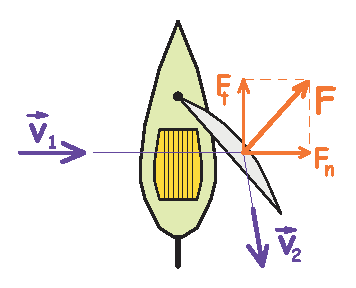
\includegraphics{GP006/GP006F10.eps}}
   \put(190,0){\makebox(0,0)[br]{\parbox{130mm}{Пример: ветер, отражаясь от косого паруса, меняет свое направление, а сила реакции давит на парус и толкает яхту вперед. Еще пример: лопатки турбины меняют направление потока газа, а сила реакции создает момент, который крутит турбину.
   }}}
  \end{picture}
  
  %\newpage
  \section{Реактивные двигатели}
  %{\bf Реактивные двигатели.}

  По закону сохранения импульса: если газ выталкивается влево, то камера сгорания (вместе с ракетой) отталкивается вправо.

  Турбореактивные двигатели (авиация): воздух для горения берется извне и нагнетается в камеру сгорания турбиной, которую крутит сам же двигатель.

  И.В.Мещерский (1859 -- 1935): теория движения тел с переменной массой.\vspace{-3mm}
  \begin{displaymath}
  \frac d{dt}(m\vec{v})=\vec{F}+\frac{dm_1}{dt}\vec{v}_1-\frac{dm_2}{dt}\vec{v}_2
  \end{displaymath}
  Конкретно для ракеты с массой $m$ и относительной скоростью выбрасывания газов $u$:\vspace{-3mm}
  \begin{displaymath}
  m\vec{a}=\vec{F}+\frac{dm}{dt}\vec{u}
  \end{displaymath}

  К.Э.Циолковский (1857 -- 1935): характеристическая скорость $V$ -- максимальная, после выработки всего топлива.
  \begin{displaymath}
  V=I\cdot\ln\left({M_1}/{M_2}\right)
  \end{displaymath}
  $M_1$ -- начальная масса, \hspace{10mm}$M_2$ -- конечная масса\\
  $I$ -- удельный импульс $\equiv$ отношение $\frac{\texttt{тяга двигателя}}{\texttt{масса топлива за секунду}}$\\
  Выход из тупика: многоступенчатые носители.\\

\section{Движение вязкой жидкости}

%  {\bf Движение вязкой жидкости}\\
    \begin{picture}(190,37)(0,0)
   %\put(0,0){\framebox(190,37)[b]{}}
   \put(0,0){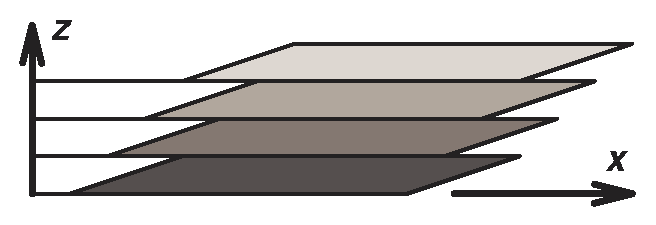
\includegraphics{GP006/GP006F11.eps}}
   \put(190,0){\makebox(0,0)[br]{\parbox{80mm}{
   Если один слой (e.g., верх\-ний) движется быстрее другого (e.g., нижнего), то между ними возникает трение (верхний тя\-нет, а нижний тормозит).
   }}}
  \end{picture}\\
  Сила внутреннего трения $f$ между слоями тем больше, чем больше площадка $\Delta S$, которую мы рассматриваем, и чем больше разница в скорости у соседних слоев (i.e., чем больше градиент скорости $\frac{dv}{dz}$):
  \begin{displaymath}
  f=\mu\frac{dv}{dz}\Delta S
  \end{displaymath}
  $\mu$ -- коэфф.внутреннего трения $\equiv$ коэффициент вязкости [Пуаз=г/см/с].\\

  \noindent
    \begin{picture}(190,90)(0,0)
   %\put(0,0){\framebox(190,90)[b]{}}
   \put(0,0){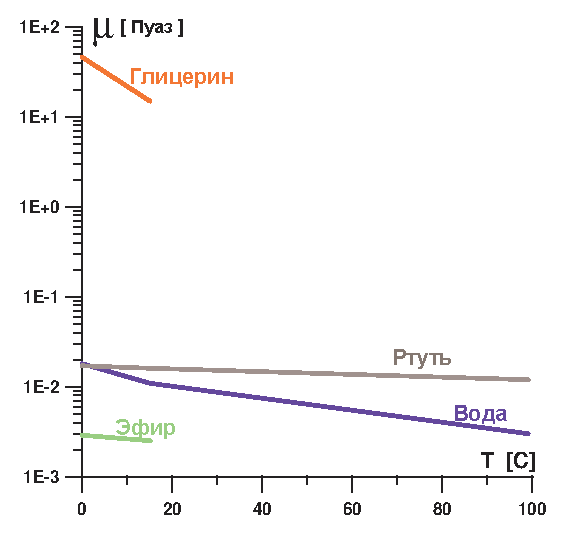
\includegraphics{GP006/GP006F12.eps}}
   \put(95,0){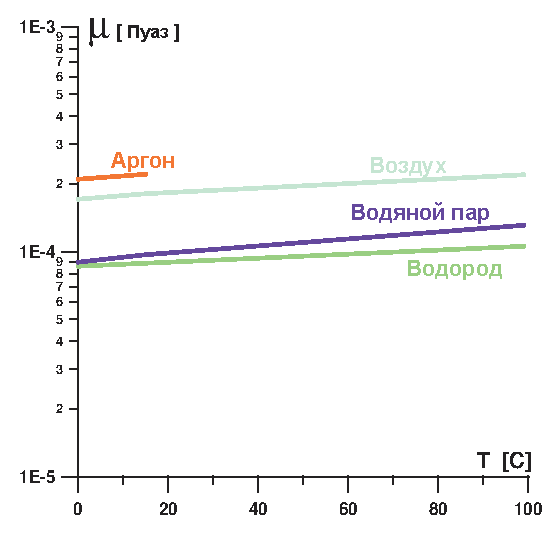
\includegraphics{GP006/GP006F13.eps}}
  \end{picture}\\

П.Л.Капица: сверхтекучесть гелия при T<-271C (<2.19K).

Л.Д.Ландау: гидродинамическая теория сверхтекучести.\\
\rule{189mm}{0.3mm}

До сих пор речь шла о ЛАМИНАРНОМ (слоистом) движении. Теперь поговорим о ТУРБУЛЕНТНОМ (когда вектор скорости беспордочно откло\-ня\-ется от среднего значения).\\
  \begin{picture}(190,50)(0,0)
   %\put(0,0){\framebox(190,50)[b]{}}
   \put(20,0){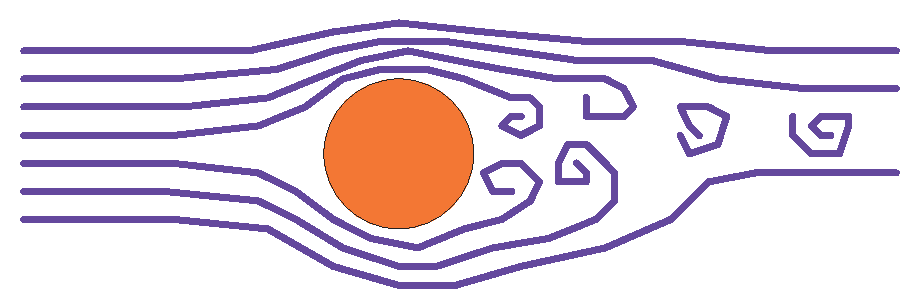
\includegraphics{GP006/GP006F14.eps}}
  \end{picture}\\
Поток распадается на отдельные вихри ({\bf вихрь = curl = rotor})

Число Рейнольдса R: $R=\frac{\rho v L}\mu$,  где $\rho$ -- плотность жидкости, $L$ -- ха\-рак\-тер\-ный поперечный размер (диаметр трубы, ширина или глубина реки, и т.п.). При $R>R_{\texttt{критич.}}$ происходит переход движения от ламинарного к турбулентному. Для воды в трубе $R_{\texttt{критич.}}\simeq$ 1200. Смысл R: работа сил трения по сравнению с кинетической энергией.

{\bf Закон Стокса} для шара в вязкой жидкости: $f=6\pi\mu r v$. Если учесть выталкивающую силу, то эффективный вес шара
\begin{displaymath}
P=(\rho_\texttt{ш}-\rho_\texttt{ж})g\frac43\pi r^3
\end{displaymath}
и для {\em установившейся скорости} падения шара в жидкости получим:
\begin{displaymath}
v=\frac{2(\rho_\texttt{ш}-\rho_\texttt{ж})g r^2}{9\mu}
\end{displaymath}
Закон Стокса выполняется только при малых значениях R. При больших R начинают появляться вихри, которые уносят большую энергию $\Rightarrow$ со\-про\-тив\-ле\-ние резко возрастает.

Подъемная сила. Н.Е.Жуковский (1847 -- 1921). Обтекание НЕСИМ\-МЕТ\-РИЧ\-НО\-ГО тела ВЯЗКОЙ жидкостью:\\
  \begin{picture}(190,57)(0,0)
   %\put(0,0){\framebox(190,60)[b]{}}
   \put(100,0){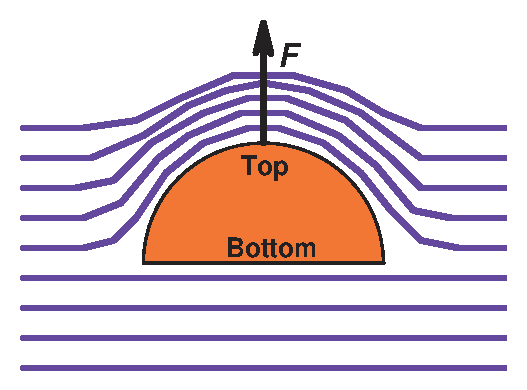
\includegraphics{GP006/GP006F15.eps}}
   \put(0,0){\makebox(0,0)[bl]{\parbox{90mm}{
   Давление внизу $p_B$ равно давлению во всей жидкости $p$, а вверху скорость должна возрасти, и потому давление (по формуле Бернулли) должно уменьшиться: $p_T<p$. Результирующая сила направлена вверх!
   }}}
  \end{picture}

  Если рассмотреть движение вязкой жидкости в круглой трубе, то мож\-но выделить цилиндрические слои. Быстрее всех движется самый цент\-раль\-ный, а медленнее -- прилегающий к стенке. Чем меньше радиус трубы -- тем больше поперечный градиент скорости и тем больше трение. Решая страшные уравнения, можно получить:
  \begin{displaymath}
  v=\frac{p_1-p_2}{4L\mu}(R^2-r^2)
  \end{displaymath}
  Здесь $L$ -- длина трубы, $R$ -- ее радиус, $p_1-p_2$ -- разность давлений на входе и выходе, $r$ -- радиус рассматриваемого слоя. Интегрируя по $r$ от 0 до $R$, найдем скорость прокачки -- объем в единицу времени:
  \begin{displaymath}
  \frac{dV}{dt}=\frac{(p_1-p_2)\pi \color{red}R^4}{8L\mu}\;\;\;\;\;\;-\texttt{формула Пуазейля}
  \end{displaymath}


